\chapter{Circuiti}

\section{Teoria dei Circuiti}  

\subsection*{Circuito}
Il circuito discerne dalla tendenza a dividere i problemi in un insieme di sottoproblemi più piccoli e facilmente comprensibili.

\subsection*{Definizione}
Un circuito è un insieme di componenti collegati fra loro tramite collegamenti (morsetti, fili o conduttori).

\subsection*{Componente}
Un componente è un elemento circuitale caratterizzato da un insieme di morsetti (I/O) e da un insieme di equazioni fra le variabili di interfaccia (relazioni costitutive) dipendenti da un numero finito di costanti numeriche (parametri circuitali).
\begin{figure}[H]
    \centering
    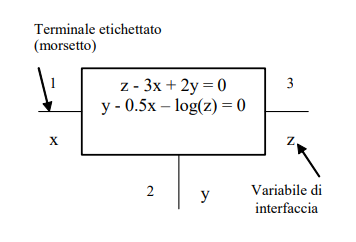
\includegraphics[width=0.5\textwidth]{capitoli/capitolo1/immagini/image1.png}
\end{figure}


\subsection*{Collegamento}
Un collegamento è un arco orientato o non che collega fra loro i morsetti dei componenti circuitali. 
Impedisce l'omogeneità e la continuità alle variabili in corrispondenza dei morsetti. 
Costituisce un'equazione di \textbf{vincolo} fra variabile e interfaccia.
L'insieme dei collegamenti può essere descritto da un grafo opportuno.

\subsection*{Sistema risolvente del circuito}
Il sistema risolvente del circuito è costituito dall'insieme delle equazioni costitutive del componente, equazioni di vincolo, condizioni iniziali e andamenti imposti da cause. 

\subsection*{Risolvere un circuito}
L'obiettivo di risolvere un circuito è calcolare gli andamenti temporali delle variabili di interfaccia. 
Questo è possibile solo se il sistema ammette una soluzione unica ogni istante di tempo.

\subsection*{Due classi di circuiti}
\subsubsection*{Circuiti non direzionali}
\begin{itemize}
    \item La direzione degli scambi è indeterminata.
    \item Non è stabilito un rapporto causa-effetto.
    \item Le variabili di interfaccia dipendono dai componenti del circuito.
    \item La tecnica di soluzione calcola tutte le variabili di interfaccia.
    \begin{figure}[H]
        \centering
        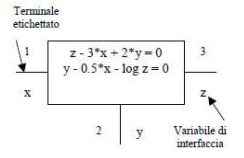
\includegraphics[width=0.5\textwidth]{capitoli/capitolo1/immagini/image2.png}
    \end{figure}
\end{itemize}

\subsubsection*{Circuiti (uni-)direzionali}
\begin{itemize}
    \item La direzione è stabilita a priori.
    \item Il funzionamento è disaccoppiato.
    \item La tecnica di soluzione calcola sequenzialmente le variabili di interfaccia.
    \begin{figure}[H]
        \centering
        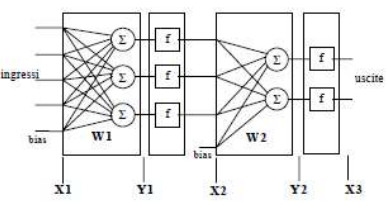
\includegraphics[width=0.7\textwidth]{capitoli/capitolo1/immagini/image3.png}
    \end{figure}
\end{itemize}

\subsection*{Variabili di interfaccia}
Le variabili di interfaccia sono grandezze (segnali) definite sui collegamenti tra componenti, sottoposte a equazioni di vincolo generate dai collegamenti e dalle equazioni dei componenti. 
Tutte le variabili sono funzioni di una o più variabili indipendenti comuni (solitamente il tempo).

\subsection*{Tipi di variabili di interfaccia}
\begin{figure}[H]
    \centering
    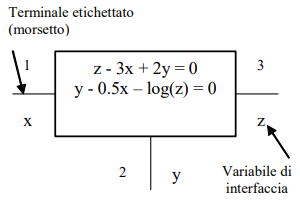
\includegraphics[width=0.7\textwidth]{capitoli/capitolo1/immagini/image4.png}
\end{figure} 
\begin{itemize}
    \item \textbf{A tempo continuo}
    \begin{itemize}
        \item Analogiche.
        \item Riproducono grandezze del mondo fisico.
        \item Hanno un valore per ogni istante \( t \).
        \item A valori reali, limitate, continue.
        \item Possono essere considerate anche a valori complessi, non continue e non limitate.
    \end{itemize}
    \item \textbf{A tempo discreto}
    \begin{itemize}
        \item Digitali.
        \item A valori discreti.
        \item Un solo valore per istanti discreti \( n \).
        \item A valori reali, limitate e continue.
        \item Possono essere considerate anche a valori complessi, non limitate.
    \end{itemize}
\end{itemize}

\section{Circuiti}

\subsection*{Circuiti analogici}
I circuiti analogici sono circuiti con variabili di interfaccia analogiche e relazioni costitutive a tempo continuo.

\subsection*{Circuito a tempo discreto}
Un circuito a tempo discreto è costituito da elementi hardware programmabili via software, con variabili di interfaccia e relazioni costitutive a tempo discreto.

\section{Approccio Circuitale}
\begin{itemize}
    \item Utilizzato per modellare fenomeni fisici diversi.
    \item Modellazione semplice e flessibile.
    \item Applicabile sia a modelli a tempo continuo che a tempo discreto.
    \item Può introdurre approssimazioni.
    \item Il limite è la frequenza e le dimensioni del circuito.
\end{itemize}
